\documentclass[11pt,a4paper]{article}
\usepackage[utf8]{inputenc}
\usepackage[T1]{fontenc}
\usepackage{geometry}
\usepackage{graphicx}
\usepackage{hyperref}
\usepackage{listings}
\usepackage{xcolor}
\usepackage{booktabs}
\usepackage{longtable}
\usepackage{array}
\usepackage{tikz}
\usepackage{fancyhdr}
\usepackage{tocloft}
\usepackage{enumitem}
\usepackage{float}
\usepackage{subcaption}
\usepackage{amsmath}
\usepackage{amssymb}
\usepackage{mdframed}
\usepackage{titlesec}

\usetikzlibrary{shapes.geometric, arrows, positioning, calc, fit, backgrounds}

\geometry{margin=1in}

% Colors
\definecolor{hydra-blue}{RGB}{5,32,73}
\definecolor{hydra-gold}{RGB}{255,199,44}
\definecolor{action-bg}{RGB}{230,247,255}
\definecolor{warning-bg}{RGB}{255,243,205}
\definecolor{success-bg}{RGB}{212,237,218}
\definecolor{info-bg}{RGB}{240,240,240}

% Hyperref setup
\hypersetup{
    colorlinks=true,
    linkcolor=hydra-blue,
    filecolor=magenta,
    urlcolor=blue,
}

% Custom environments
\newmdenv[
    backgroundcolor=action-bg,
    linecolor=hydra-blue,
    linewidth=2pt,
    topline=false,
    bottomline=false,
    rightline=false,
    skipabove=\topsep,
    skipbelow=\topsep,
    innertopmargin=10pt,
    innerbottommargin=10pt,
]{actionbox}

\newmdenv[
    backgroundcolor=warning-bg,
    linecolor=orange,
    linewidth=2pt,
    topline=false,
    bottomline=false,
    rightline=false,
    skipabove=\topsep,
    skipbelow=\topsep,
]{warningbox}

\newmdenv[
    backgroundcolor=success-bg,
    linecolor=green!50!black,
    linewidth=2pt,
    topline=false,
    bottomline=false,
    rightline=false,
    skipabove=\topsep,
    skipbelow=\topsep,
]{successbox}

% Header/Footer
\pagestyle{fancy}
\fancyhf{}
\fancyhead[L]{\textcolor{hydra-blue}{\textbf{Hydra Infrastructure Proposal}}}
\fancyhead[R]{\textcolor{hydra-blue}{SUNY New Paltz}}
\fancyfoot[C]{\thepage}
\renewcommand{\headrulewidth}{0.4pt}
\renewcommand{\footrulewidth}{0.4pt}

% Section formatting
\titleformat{\section}
{\color{hydra-blue}\normalfont\Large\bfseries}
{\thesection}{1em}{}

\titleformat{\subsection}
{\color{hydra-blue}\normalfont\large\bfseries}
{\thesubsection}{1em}{}

\begin{document}

% Title Page
\begin{titlepage}
\centering
\vspace*{2cm}

{\Huge\bfseries\color{hydra-blue} Hydra Lab Infrastructure Proposal\par}
\vspace{0.5cm}
{\Large Storage \& GPU Cluster Modernization\par}

\vspace{2cm}

{\large Computer Science Department\\SUNY New Paltz\par}

\vspace{1cm}

{\large\today\par}

\vfill

\begin{abstract}
This proposal outlines the infrastructure modernization plan for the Hydra computing cluster, including ZFS RAID-10 storage deployment, GPU node optimization, multi-node inference setup, and Kubernetes orchestration. The plan addresses current storage limitations, optimizes GPU utilization across heterogeneous hardware, and establishes a scalable foundation for student container workloads.
\end{abstract}

\end{titlepage}

\tableofcontents
\newpage

% =============================================================================
\section{Executive Summary}
% =============================================================================

\subsection{Current State}
The Hydra Lab currently operates three servers with underutilized storage capacity and suboptimal GPU resource allocation. Student containers run on limited local storage, and GPU access requires manual intervention.

\subsection{Proposed Changes}
\begin{itemize}
    \item Deploy 21TB ZFS RAID-10 storage pool on Hydra for centralized container storage
    \item Optimize GPU node storage to leverage fast NVMe drives for model inference
    \item Implement multi-node Ollama deployment for distributed inference (136GB VRAM)
    \item Deploy RKE2 Kubernetes cluster for automated GPU scheduling
    \item Establish centralized logging and monitoring infrastructure
\end{itemize}

\subsection{Expected Outcomes}
\begin{itemize}
    \item 21TB redundant storage with automatic compression and snapshots
    \item 5$\times$ GPU utilization improvement through intelligent scheduling
    \item Reduced manual intervention for student GPU access requests
    \item Foundation for future expansion and self-service portal
\end{itemize}

% =============================================================================
\section{Hardware Inventory}
% =============================================================================

\subsection{Cluster Overview}

\begin{table}[H]
\centering
\caption{Cluster Hardware Configuration}
\begin{tabular}{@{}lcccp{5cm}@{}}
\toprule
\textbf{Node} & \textbf{Role} & \textbf{RAM} & \textbf{GPUs} & \textbf{Storage} \\
\midrule
Hydra & Control + Storage & 251GB & None & 6$\times$7TB RAID-10, 1.7TB OS, 1.1TB backup \\
Chimera & GPU Inference & 251GB & 3$\times$RTX 3090 (72GB) & 3.5TB NVMe (fast), 3.5TB SATA (slow) \\
Cerberus & GPU Training & 64GB & 2$\times$RTX 5090 (64GB) & 3.6TB NVMe, 1.7TB NVMe \\
\bottomrule
\end{tabular}
\end{table}

\subsection{Hydra Storage Drives}

\begin{table}[H]
\centering
\begin{tabular}{@{}lllll@{}}
\toprule
\textbf{Device} & \textbf{Size} & \textbf{Model} & \textbf{Speed} & \textbf{Purpose} \\
\midrule
sda-sdf & 7TB each & PA33N7T6 EMC7680 & 550-750 MB/s & RAID-10 pool (tank) \\
sdg & 1.7TB & Micron MTFDDAK1T9TDS & 548 MB/s & OS boot drive \\
sdh & 1.1TB & Seagate ST1200MM0099 & 255 MB/s & Daily OS backups \\
\bottomrule
\end{tabular}
\end{table}

\begin{warningbox}
\textbf{Note:} The 1.1TB Seagate drive (sdh) is labeled as "SAS 10k" but benchmarks at only 255 MB/s—likely a mislabeled SATA drive. Suitable for cold backups only, not as ZFS cache.
\end{warningbox}

\subsection{Chimera Storage Drives}

\begin{table}[H]
\centering
\begin{tabular}{@{}lllll@{}}
\toprule
\textbf{Device} & \textbf{Size} & \textbf{Model} & \textbf{Speed} & \textbf{Purpose} \\
\midrule
nvme0n1 & 3.5TB & Samsung MZ1L23T8HBLA & 2.2 GB/s & OS + Ollama models \\
sda & 3.5TB & Micron 5210 & \textcolor{red}{19 MB/s} & Cold storage only \\
\bottomrule
\end{tabular}
\end{table}

\begin{warningbox}
\textbf{Critical:} The Micron 5210 (sda) benchmarks at only 19 MB/s—extremely slow. All active workloads must use the NVMe drive. The SATA drive is suitable only for archives and cold backups.
\end{warningbox}

\subsection{Cerberus Storage Drives}

\begin{table}[H]
\centering
\begin{tabular}{@{}lllll@{}}
\toprule
\textbf{Device} & \textbf{Size} & \textbf{Model} & \textbf{Speed} & \textbf{Purpose} \\
\midrule
nvme0n1 & 3.6TB & MSI M480 PRO & 2.5 GB/s & OS + containers \\
nvme1n1 & 1.7TB & Samsung MZQL21T9HCJR & 2.5 GB/s & Model storage \\
\bottomrule
\end{tabular}
\end{table}

% =============================================================================
\section{Architecture Overview}
% =============================================================================

\subsection{Target Architecture}

\begin{figure}[H]
\centering
\resizebox{\textwidth}{!}{%
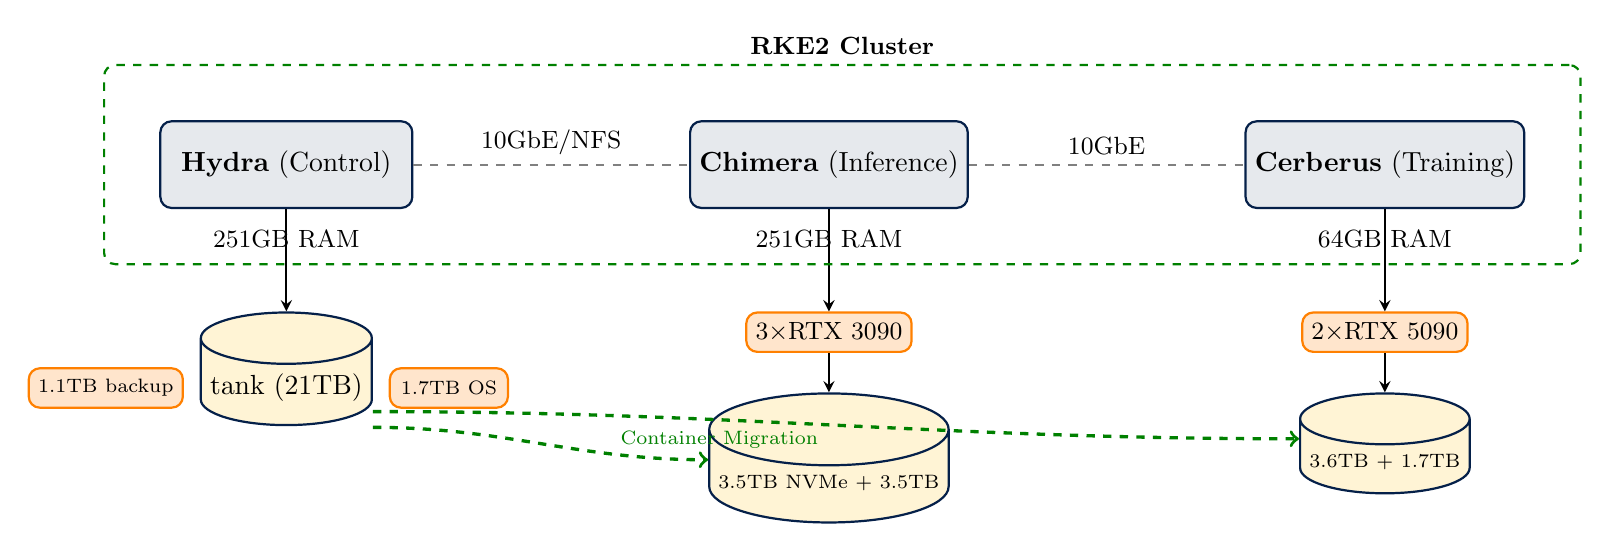
\begin{tikzpicture}[
    node distance=2cm,
    server/.style={rectangle, draw=hydra-blue, thick, minimum width=3.2cm, minimum height=1.1cm, fill=hydra-blue!10, rounded corners},
    storage/.style={cylinder, draw=hydra-blue, thick, minimum width=1.8cm, minimum height=0.9cm, fill=hydra-gold!20, shape border rotate=90, aspect=0.3},
    cache/.style={rectangle, draw=orange, thick, minimum width=1.5cm, minimum height=0.5cm, fill=orange!20, rounded corners, font=\scriptsize},
    gpu/.style={rectangle, draw=orange, thick, minimum width=1.4cm, minimum height=0.5cm, fill=orange!20, rounded corners, font=\small},
    network/.style={draw=gray, thick, dashed},
    migration/.style={draw=green!50!black, very thick, dashed, ->},
    arrow/.style={->, >=stealth, thick}
]

% Hydra
\node[server] (hydra) {\textbf{Hydra} (Control)};
\node[below=0.15cm of hydra, font=\small] (hydra-ram) {251GB RAM};
\node[storage, below=1.3cm of hydra] (tank) {tank (21TB)};
\node[cache, left=0.2cm of tank] (backup) {1.1TB backup};
\node[cache, right=0.2cm of tank] (boot) {1.7TB OS};
\draw[arrow] (hydra) -- (tank);

% Chimera
\node[server, right=3.5cm of hydra] (chimera) {\textbf{Chimera} (Inference)};
\node[below=0.15cm of chimera, font=\small] (chimera-ram) {251GB RAM};
\node[gpu, below=1.3cm of chimera] (gpu1) {3$\times$RTX 3090};
\node[storage, below=0.5cm of gpu1, font=\scriptsize] (cnvme) {3.5TB NVMe + 3.5TB};
\draw[arrow] (chimera) -- (gpu1);
\draw[arrow] (gpu1) -- (cnvme);

% Cerberus
\node[server, right=3.5cm of chimera] (cerberus) {\textbf{Cerberus} (Training)};
\node[below=0.15cm of cerberus, font=\small] (cerb-ram) {64GB RAM};
\node[gpu, below=1.3cm of cerberus] (gpu2) {2$\times$RTX 5090};
\node[storage, below=0.5cm of gpu2, font=\scriptsize] (cenvme) {3.6TB + 1.7TB};
\draw[arrow] (cerberus) -- (gpu2);
\draw[arrow] (gpu2) -- (cenvme);

% Network connections
\draw[network] (hydra.east) -- (chimera.west) node[midway, above, font=\small] {10GbE/NFS};
\draw[network] (chimera.east) -- (cerberus.west) node[midway, above, font=\small] {10GbE};

% Container migration paths
\draw[migration] ([yshift=-0.5cm]tank.east) to[out=0,in=180] ([yshift=0.3cm]cnvme.west);
\draw[migration] ([yshift=-0.3cm]tank.east) to[out=0,in=180] ([yshift=0.3cm]cenvme.west);
\node[font=\scriptsize, text=green!50!black] at (5.5,-3.5) {Container Migration};

% Kubernetes overlay
\node[draw=green!50!black, thick, dashed, fit=(hydra)(chimera)(cerberus), inner sep=0.7cm, rounded corners, label={[font=\small\bfseries]above:RKE2 Cluster}] {};

\end{tikzpicture}%
}
\caption{Target Cluster Architecture}
\end{figure}

\subsection{Storage Architecture}

\begin{figure}[H]
\centering
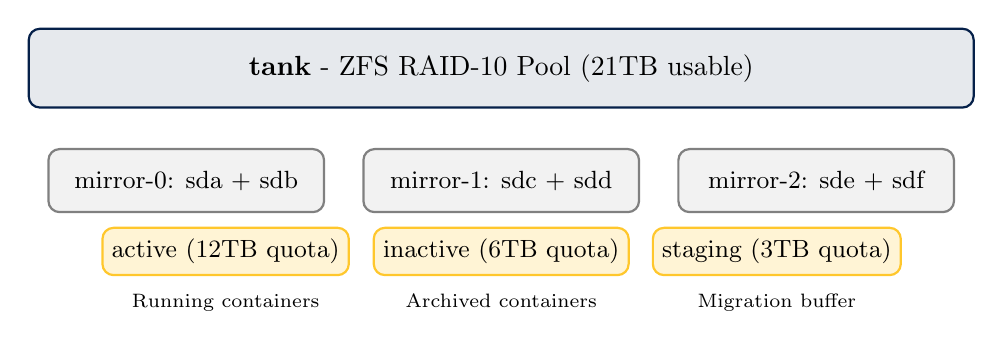
\begin{tikzpicture}[
    node distance=0.3cm,
    pool/.style={rectangle, draw=hydra-blue, thick, minimum width=12cm, minimum height=1cm, fill=hydra-blue!10, rounded corners},
    vdev/.style={rectangle, draw=gray, thick, minimum width=3.5cm, minimum height=0.8cm, fill=gray!10, rounded corners, font=\small},
    dataset/.style={rectangle, draw=hydra-gold, thick, minimum width=3cm, minimum height=0.6cm, fill=hydra-gold!20, rounded corners, font=\small},
]

% Pool
\node[pool] (tank) {\textbf{tank} - ZFS RAID-10 Pool (21TB usable)};

% Mirror vdevs
\node[vdev, below=0.5cm of tank, xshift=-4cm] (m1) {mirror-0: sda + sdb};
\node[vdev, below=0.5cm of tank] (m2) {mirror-1: sdc + sdd};
\node[vdev, below=0.5cm of tank, xshift=4cm] (m3) {mirror-2: sde + sdf};

% Datasets
\node[dataset, below=1.5cm of tank, xshift=-3.5cm] (active) {active (12TB quota)};
\node[dataset, below=1.5cm of tank] (inactive) {inactive (6TB quota)};
\node[dataset, below=1.5cm of tank, xshift=3.5cm] (staging) {staging (3TB quota)};

% Labels
\node[font=\scriptsize, below=0.1cm of active] {Running containers};
\node[font=\scriptsize, below=0.1cm of inactive] {Archived containers};
\node[font=\scriptsize, below=0.1cm of staging] {Migration buffer};

\end{tikzpicture}
\caption{ZFS Storage Pool Architecture}
\end{figure}

% =============================================================================
\section{Phase 0: Pre-Migration Backup}
% =============================================================================

\subsection{Overview}
Before making any changes to the cluster, all critical data will be backed up to Chimera's slow /data drive (3.5TB Micron). This drive is only 19 MB/s but adequate for one-time backups.

\begin{warningbox}
\textbf{Critical:} All backups must be completed and verified before proceeding to Phase 1.
\end{warningbox}

\subsection{Backup Actions}

\begin{actionbox}
\textbf{0.1 Prepare Backup Location}
\begin{itemize}[noitemsep]
    \item Verify Chimera /data has sufficient space ($\sim$3.5TB available)
    \item Create backup directory structure at /data/backups/
    \item Create subdirectories for hydra, chimera, cerberus
\end{itemize}
\end{actionbox}

\begin{actionbox}
\textbf{0.2 Backup Hydra}
\begin{itemize}[noitemsep]
    \item Backup /home directories (user data) via rsync over network
    \item Backup /etc configuration files
    \item Backup Docker volumes from /var/lib/docker/volumes/
    \item Dump MySQL databases to SQL file
    \item Dump PostgreSQL databases to SQL file
\end{itemize}
\end{actionbox}

\begin{actionbox}
\textbf{0.3 Backup Chimera}
\begin{itemize}[noitemsep]
    \item Backup /home directories locally
    \item Backup /etc configuration files
    \item Backup Ollama models from /var/lib/ollama/
    \item Backup Docker volumes
    \item Dump MySQL databases if present
\end{itemize}
\end{actionbox}

\begin{actionbox}
\textbf{0.4 Backup Cerberus}
\begin{itemize}[noitemsep]
    \item Backup /home directories via rsync over network
    \item Backup /etc configuration files
\end{itemize}
\end{actionbox}

\begin{actionbox}
\textbf{0.5 Verify Backups}
\begin{itemize}[noitemsep]
    \item Check backup sizes with du -sh /data/backups/*/
    \item Verify critical files exist in each backup directory
    \item Test database dumps are valid SQL
    \item Confirm total backup size fits on /data
\end{itemize}
\end{actionbox}

% =============================================================================
\section{Phase 1: ZFS Storage Setup on Hydra}
% =============================================================================

\subsection{Overview}
Deploy a ZFS RAID-10 pool using 6$\times$7TB enterprise drives in 3 mirror pairs, providing 21TB usable storage with redundancy (can lose one drive per mirror pair).

\subsection{Storage Actions}

\begin{actionbox}
\textbf{1.1 Verify Hardware}
\begin{itemize}[noitemsep]
    \item Confirm 6$\times$7TB drives (sda-sdf) are detected
    \item Verify drives are PA33N7T6 EMC7680 model
    \item Check drive health with smartctl
\end{itemize}
\end{actionbox}

\begin{actionbox}
\textbf{1.2 Install ZFS}
\begin{itemize}[noitemsep]
    \item Install zfsutils-linux package
    \item Load ZFS kernel modules
    \item Verify installation with zfs version
\end{itemize}
\end{actionbox}

\begin{actionbox}
\textbf{1.3 Create RAID-10 Pool}
\begin{itemize}[noitemsep]
    \item Create pool "tank" with 3 mirror vdevs
    \item Mirror pair 1: sda + sdb
    \item Mirror pair 2: sdc + sdd
    \item Mirror pair 3: sde + sdf
    \item Set ashift=12 for 4K sector alignment
    \item Enable lz4 compression
    \item Disable atime for performance
\end{itemize}
\end{actionbox}

\begin{actionbox}
\textbf{1.4 Create Datasets}
\begin{itemize}[noitemsep]
    \item Create tank/active with 12TB quota (running containers)
    \item Create tank/inactive with 6TB quota (archived containers)
    \item Create tank/staging with 3TB quota (migration buffer)
\end{itemize}
\end{actionbox}

\begin{actionbox}
\textbf{1.5 Configure Backup Drive}
\begin{itemize}[noitemsep]
    \item Format sdh (1.1TB Seagate) as ext4
    \item Mount at /backups
    \item Add to /etc/fstab for persistence
    \item Create backup subdirectories for each node
\end{itemize}
\end{actionbox}

\begin{actionbox}
\textbf{1.6 Configure NFS Exports}
\begin{itemize}[noitemsep]
    \item Install nfs-kernel-server
    \item Export /tank/active to 192.168.1.0/24
    \item Export /tank/inactive to 192.168.1.0/24
    \item Export /tank/staging to 192.168.1.0/24
    \item Set rw,async,no\_root\_squash options
\end{itemize}
\end{actionbox}

\begin{actionbox}
\textbf{1.7 Setup Automatic Snapshots}
\begin{itemize}[noitemsep]
    \item Configure hourly snapshots of tank/active (retain 24)
    \item Configure daily snapshots of all datasets (retain 7)
    \item Schedule weekly scrub on Sundays at 1 AM
\end{itemize}
\end{actionbox}

\begin{actionbox}
\textbf{1.8 Setup Daily OS Backups}
\begin{itemize}[noitemsep]
    \item Create backup script at /usr/local/bin/backup-os.sh
    \item Backup Hydra /etc and /home to /backups/hydra/
    \item Backup Chimera /etc via rsync to /backups/chimera/
    \item Backup Cerberus /etc via rsync to /backups/cerberus/
    \item Schedule via cron at 3 AM daily
\end{itemize}
\end{actionbox}

\begin{actionbox}
\textbf{1.9 Setup Cluster Aliases}
\begin{itemize}[noitemsep]
    \item Create /etc/profile.d/hydra-aliases.sh on all nodes
    \item Add SSH shortcuts: hydra, chimera, cerberus
    \item Add status aliases: gpu, gpuw, zstat, zlist, dps
    \item Add kubectl aliases: kgn, kgp
    \item Add log aliases: logs-backup, logs-docker, logs-ollama
\end{itemize}
\end{actionbox}

\begin{actionbox}
\textbf{1.10 Setup Centralized Logging}
\begin{itemize}[noitemsep]
    \item Configure rsyslog on Chimera/Cerberus to forward to Hydra
    \item Enable UDP reception on Hydra port 514
    \item Create log directories at /var/log/hydra-cluster/
    \item Logs will be used for future dashboard integration
\end{itemize}
\end{actionbox}

\subsection{Phase 1 Verification}

\begin{successbox}
\textbf{Success Criteria:}
\begin{itemize}[noitemsep]
    \item Pool status shows ONLINE with 3 mirror vdevs
    \item All datasets created with correct quotas
    \item NFS exports accessible from Chimera and Cerberus
    \item Backup drive mounted at /backups
    \item Aliases working on all nodes
\end{itemize}
\end{successbox}

% =============================================================================
\section{Phase 2: GPU Node Storage Configuration}
% =============================================================================

\subsection{Overview}
Optimize storage on both GPU nodes to ensure Ollama models run on fast NVMe storage, not slow SATA drives.

\subsection{GPU Node Storage Layout}

\begin{figure}[H]
\centering
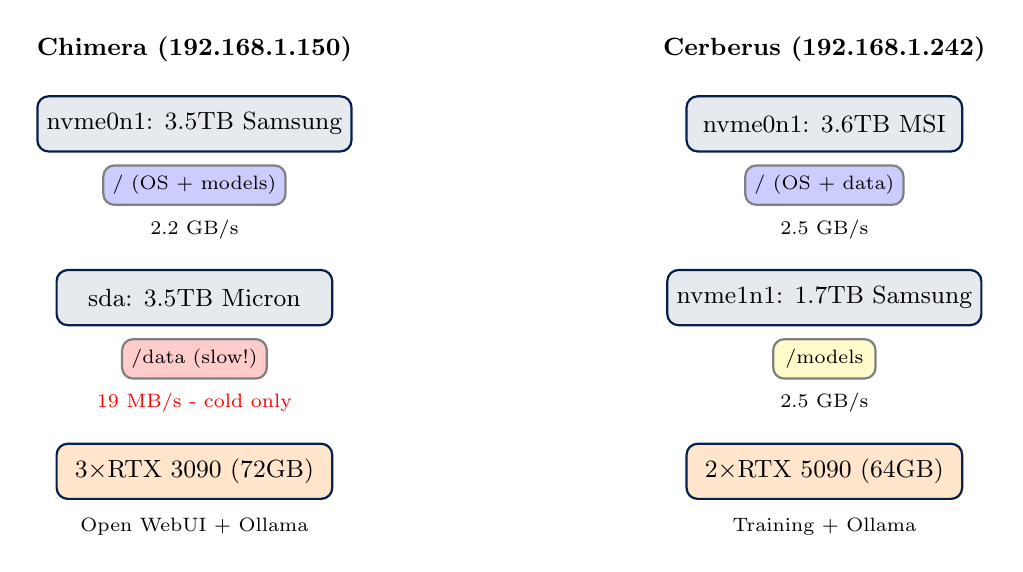
\begin{tikzpicture}[
    node distance=0.5cm,
    box/.style={rectangle, draw=hydra-blue, thick, minimum width=3.5cm, minimum height=0.7cm, fill=hydra-blue!10, rounded corners, font=\small},
    partition/.style={rectangle, draw=gray, thick, minimum width=1.3cm, minimum height=0.5cm, rounded corners, font=\scriptsize},
    label/.style={font=\small\bfseries}
]

% Chimera (left side)
\node[label] (chimera-label) at (0,0) {Chimera (192.168.1.150)};
\node[box, below=0.3cm of chimera-label] (c-nvme) {nvme0n1: 3.5TB Samsung};
\node[partition, below=0.15cm of c-nvme, fill=blue!20] (c-os) {/ (OS + models)};
\node[font=\scriptsize, below=0.05cm of c-os] {2.2 GB/s};

\node[box, below=0.8cm of c-os] (c-sda) {sda: 3.5TB Micron};
\node[partition, below=0.15cm of c-sda, fill=red!20] (c-data) {/data (slow!)};
\node[font=\scriptsize, below=0.05cm of c-data, text=red] {19 MB/s - cold only};

\node[box, below=0.8cm of c-data, fill=orange!20] (c-gpu) {3$\times$RTX 3090 (72GB)};
\node[font=\scriptsize, below=0.1cm of c-gpu] {Open WebUI + Ollama};

% Cerberus (right side)
\node[label] (cerberus-label) at (8,0) {Cerberus (192.168.1.242)};
\node[box, below=0.3cm of cerberus-label] (ce-nvme1) {nvme0n1: 3.6TB MSI};
\node[partition, below=0.15cm of ce-nvme1, fill=blue!20] (ce-os) {/ (OS + data)};
\node[font=\scriptsize, below=0.05cm of ce-os] {2.5 GB/s};

\node[box, below=0.8cm of ce-os] (ce-nvme2) {nvme1n1: 1.7TB Samsung};
\node[partition, below=0.15cm of ce-nvme2, fill=yellow!20] (ce-models) {/models};
\node[font=\scriptsize, below=0.05cm of ce-models] {2.5 GB/s};

\node[box, below=0.8cm of ce-models, fill=orange!20] (ce-gpu) {2$\times$RTX 5090 (64GB)};
\node[font=\scriptsize, below=0.1cm of ce-gpu] {Training + Ollama};

\end{tikzpicture}
\caption{GPU Node Storage Layout}
\end{figure}

\subsection{Phase 2A: Chimera Configuration}

\begin{actionbox}
\textbf{2A.1 Verify Chimera Drives}
\begin{itemize}[noitemsep]
    \item Confirm nvme0n1 (3.5TB Samsung) is mounted at /
    \item Confirm sda (3.5TB Micron) is mounted at /data
    \item Test drive speeds with hdparm
    \item Verify NVMe is $\sim$2.2 GB/s, SATA is only $\sim$19 MB/s
\end{itemize}
\end{actionbox}

\begin{warningbox}
\textbf{Important:} Do NOT store Ollama models on /data—the Micron 5210 is only 19 MB/s. All models must be stored on the fast NVMe root partition.
\end{warningbox}

\begin{actionbox}
\textbf{2A.2 Configure Ollama on Fast NVMe}
\begin{itemize}[noitemsep]
    \item Create model directory at /var/lib/ollama/models
    \item Set ownership to ollama:ollama
    \item Configure systemd override for OLLAMA\_MODELS path
    \item Configure OLLAMA\_HOST=0.0.0.0 for network access
    \item Restart ollama service
\end{itemize}
\end{actionbox}

\begin{actionbox}
\textbf{2A.3 Configure Chimera Directories}
\begin{itemize}[noitemsep]
    \item Create /var/lib/containers/\{staging,active\} on NVMe
    \item Set ownership to root:docker
    \item Use /data only for cold storage (archives, old backups)
\end{itemize}
\end{actionbox}

\begin{actionbox}
\textbf{2A.4 Verify NVIDIA Drivers}
\begin{itemize}[noitemsep]
    \item Check nvidia-smi shows 3$\times$RTX 3090
    \item Install nvidia-driver-550 if not present
    \item Enable nvidia-persistenced service
\end{itemize}
\end{actionbox}

\subsection{Phase 2B: Cerberus Configuration}

\begin{actionbox}
\textbf{2B.1 Verify Cerberus Drives}
\begin{itemize}[noitemsep]
    \item Confirm nvme0n1 (3.6TB MSI) is mounted at /
    \item Confirm nvme1n1 (1.7TB Samsung) is available for /models
\end{itemize}
\end{actionbox}

\begin{actionbox}
\textbf{2B.2 Configure Model Storage}
\begin{itemize}[noitemsep]
    \item Format nvme1n1 as ext4 with label "models"
    \item Create mount point at /models
    \item Add to /etc/fstab for persistence
    \item Create subdirectories: ollama, huggingface, checkpoints
\end{itemize}
\end{actionbox}

\begin{actionbox}
\textbf{2B.3 Configure Container Directories}
\begin{itemize}[noitemsep]
    \item Create /var/lib/containers/\{staging,active,training\}
    \item Set ownership to root:docker
\end{itemize}
\end{actionbox}

\begin{actionbox}
\textbf{2B.4 Verify NVIDIA Drivers}
\begin{itemize}[noitemsep]
    \item Check nvidia-smi shows 2$\times$RTX 5090
    \item Install nvidia-driver-550 (or 560+ for 5090 support)
    \item Enable nvidia-persistenced service
\end{itemize}
\end{actionbox}

\begin{actionbox}
\textbf{2B.5 Configure Ollama}
\begin{itemize}[noitemsep]
    \item Configure systemd override for OLLAMA\_MODELS=/models/ollama
    \item Configure OLLAMA\_HOST=0.0.0.0 for network access
    \item Restart ollama service
\end{itemize}
\end{actionbox}

\subsection{Phase 2 Verification}

\begin{successbox}
\textbf{Chimera Success Criteria:}
\begin{itemize}[noitemsep]
    \item nvme0n1 mounted at / with $\sim$2.2 GB/s
    \item sda mounted at /data (cold storage only)
    \item 3$\times$RTX 3090 detected by nvidia-smi
    \item Ollama using /var/lib/ollama/models on fast NVMe
\end{itemize}
\end{successbox}

\begin{successbox}
\textbf{Cerberus Success Criteria:}
\begin{itemize}[noitemsep]
    \item nvme0n1 mounted at /
    \item nvme1n1 mounted at /models
    \item 2$\times$RTX 5090 detected by nvidia-smi
    \item Ollama using /models/ollama
\end{itemize}
\end{successbox}

% =============================================================================
\section{Phase 2C: Open WebUI Multi-Node Setup}
% =============================================================================

\subsection{Overview}
Deploy Open WebUI on Chimera with connections to Ollama instances on both GPU nodes, providing 136GB total VRAM (72GB + 64GB) for inference workloads.

\begin{figure}[H]
\centering
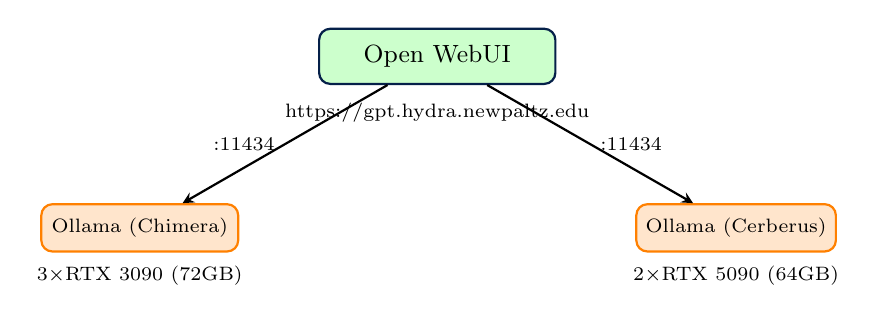
\begin{tikzpicture}[
    node distance=1cm,
    box/.style={rectangle, draw=hydra-blue, thick, minimum width=3cm, minimum height=0.7cm, fill=hydra-blue!10, rounded corners, font=\small},
    ollama/.style={rectangle, draw=orange, thick, minimum width=2.5cm, minimum height=0.6cm, fill=orange!20, rounded corners, font=\scriptsize},
    arrow/.style={->, >=stealth, thick}
]

% Open WebUI
\node[box, fill=green!20] (webui) {Open WebUI};
\node[font=\scriptsize, below=0.1cm of webui] {https://gpt.hydra.newpaltz.edu};

% Ollama instances
\node[ollama, below left=1.5cm and 1cm of webui] (ollama1) {Ollama (Chimera)};
\node[font=\scriptsize, below=0.05cm of ollama1] {3$\times$RTX 3090 (72GB)};

\node[ollama, below right=1.5cm and 1cm of webui] (ollama2) {Ollama (Cerberus)};
\node[font=\scriptsize, below=0.05cm of ollama2] {2$\times$RTX 5090 (64GB)};

% Arrows
\draw[arrow] (webui) -- (ollama1) node[midway, left, font=\scriptsize] {:11434};
\draw[arrow] (webui) -- (ollama2) node[midway, right, font=\scriptsize] {:11434};

\end{tikzpicture}
\caption{Open WebUI Multi-Node Architecture (136GB VRAM)}
\end{figure}

\subsection{Multi-Node Setup Actions}

\begin{actionbox}
\textbf{2C.1 Install Ollama on Chimera}
\begin{itemize}[noitemsep]
    \item Install Ollama via official install script
    \item Configure OLLAMA\_MODELS to /var/lib/ollama/models (fast NVMe)
    \item Configure OLLAMA\_HOST=0.0.0.0 for network access
    \item Enable and start ollama service
\end{itemize}
\end{actionbox}

\begin{actionbox}
\textbf{2C.2 Install Ollama on Cerberus}
\begin{itemize}[noitemsep]
    \item Install Ollama via official install script
    \item Configure OLLAMA\_MODELS to /models/ollama
    \item Configure OLLAMA\_HOST=0.0.0.0 for network access
    \item Enable and start ollama service
\end{itemize}
\end{actionbox}

\begin{actionbox}
\textbf{2C.3 Pull Models}
\begin{itemize}[noitemsep]
    \item On Chimera (inference): llama3.1:70b, codellama:34b, mistral
    \item On Cerberus (training): llama3.1:70b, deepseek-coder:33b
\end{itemize}
\end{actionbox}

\begin{actionbox}
\textbf{2C.4 Configure Open WebUI}
\begin{itemize}[noitemsep]
    \item Update docker-compose.yml on Chimera
    \item Set OLLAMA\_BASE\_URLS to include both localhost:11434 and cerberus:11434
    \item Enable WEBUI\_AUTH for authentication
    \item Restart Open WebUI container
\end{itemize}
\end{actionbox}

\subsection{Model Distribution Strategy}

\begin{table}[H]
\centering
\caption{Recommended Model Placement}
\begin{tabular}{@{}llp{6cm}@{}}
\toprule
\textbf{Node} & \textbf{Models} & \textbf{Rationale} \\
\midrule
Chimera (72GB) & llama3.1:70b, codellama:34b, mistral & Primary inference, lower latency \\
Cerberus (64GB) & llama3.1:70b, deepseek-coder, fine-tunes & Training workloads, large batches \\
\bottomrule
\end{tabular}
\end{table}

\begin{successbox}
\textbf{Load Balancing:} Open WebUI automatically distributes requests across available Ollama instances. If Cerberus is busy with training, requests route to Chimera.
\end{successbox}

% =============================================================================
\section{Phase 3: RKE2 Kubernetes Deployment}
% =============================================================================

\subsection{Overview}
Deploy RKE2 (Rancher Kubernetes Engine 2) across all three nodes with Hydra as the control plane and Chimera/Cerberus as GPU workers.

\subsection{Why RKE2 over Docker Swarm}

\begin{table}[H]
\centering
\caption{RKE2 vs Docker Swarm Comparison}
\begin{tabular}{@{}lcc@{}}
\toprule
\textbf{Feature} & \textbf{RKE2} & \textbf{Docker Swarm} \\
\midrule
GPU Scheduling & Native NVIDIA plugin & Manual placement \\
Resource Limits & Fine-grained (millicores) & Basic \\
Heterogeneous GPUs & Node selectors/taints & Difficult \\
Container Isolation & Pod security policies & Limited \\
SAML/OIDC Auth & Native support & External tools \\
Production Grade & CNCF certified & Community only \\
\bottomrule
\end{tabular}
\end{table}

\subsection{Cluster Topology}

\begin{table}[H]
\centering
\caption{RKE2 Cluster Configuration}
\begin{tabular}{@{}llll@{}}
\toprule
\textbf{Node} & \textbf{Role} & \textbf{Labels} & \textbf{Taints} \\
\midrule
Hydra & Server (control plane) & role=control & -- \\
Chimera & Agent (GPU worker) & gpu-type=rtx3090, gpu-count=3 & -- \\
Cerberus & Agent (GPU worker) & gpu-type=rtx5090, gpu-count=2 & training=true:NoSchedule \\
\bottomrule
\end{tabular}
\end{table}

\subsection{RKE2 Deployment Actions}

\begin{actionbox}
\textbf{3.1 Install RKE2 Server on Hydra}
\begin{itemize}[noitemsep]
    \item Download RKE2 installer
    \item Configure /etc/rancher/rke2/config.yaml
    \item Set node-name, tls-san, disable servicelb (use MetalLB)
    \item Enable and start rke2-server service
\end{itemize}
\end{actionbox}

\begin{actionbox}
\textbf{3.2 Install RKE2 Agent on Chimera}
\begin{itemize}[noitemsep]
    \item Download RKE2 agent installer
    \item Configure server URL to point to Hydra
    \item Set node-label: gpu-type=rtx3090, gpu-count=3
    \item Copy node token from Hydra
    \item Enable and start rke2-agent service
\end{itemize}
\end{actionbox}

\begin{actionbox}
\textbf{3.3 Install RKE2 Agent on Cerberus}
\begin{itemize}[noitemsep]
    \item Download RKE2 agent installer
    \item Configure server URL to point to Hydra
    \item Set node-label: gpu-type=rtx5090, gpu-count=2
    \item Set node-taint: training=true:NoSchedule
    \item Copy node token from Hydra
    \item Enable and start rke2-agent service
\end{itemize}
\end{actionbox}

\begin{actionbox}
\textbf{3.4 Configure kubectl Access}
\begin{itemize}[noitemsep]
    \item Copy kubeconfig from /etc/rancher/rke2/rke2.yaml
    \item Set KUBECONFIG environment variable
    \item Verify with kubectl get nodes
\end{itemize}
\end{actionbox}

\begin{actionbox}
\textbf{3.5 Install NVIDIA Device Plugin}
\begin{itemize}[noitemsep]
    \item Deploy NVIDIA k8s-device-plugin DaemonSet
    \item Verify GPUs detected with kubectl describe nodes
\end{itemize}
\end{actionbox}

\subsection{Phase 3 Verification}

\begin{successbox}
\textbf{Success Criteria:}
\begin{itemize}[noitemsep]
    \item All 3 nodes show Ready status
    \item Chimera shows nvidia.com/gpu: 3
    \item Cerberus shows nvidia.com/gpu: 2
    \item System pods running in kube-system namespace
\end{itemize}
\end{successbox}

% =============================================================================
\section{GPU Job Scheduling}
% =============================================================================

\subsection{Scheduling Strategy}

\begin{table}[H]
\centering
\caption{GPU Request Routing}
\begin{tabular}{@{}llp{6cm}@{}}
\toprule
\textbf{Request Type} & \textbf{Target Node} & \textbf{Policy} \\
\midrule
Training jobs & Cerberus & Never interrupt running jobs \\
Inference requests & Chimera & Route if <50\% utilization \\
Default containers & Hydra & CPU-only, no GPU \\
\bottomrule
\end{tabular}
\end{table}

\subsection{Container Migration Flow}

\begin{figure}[H]
\centering
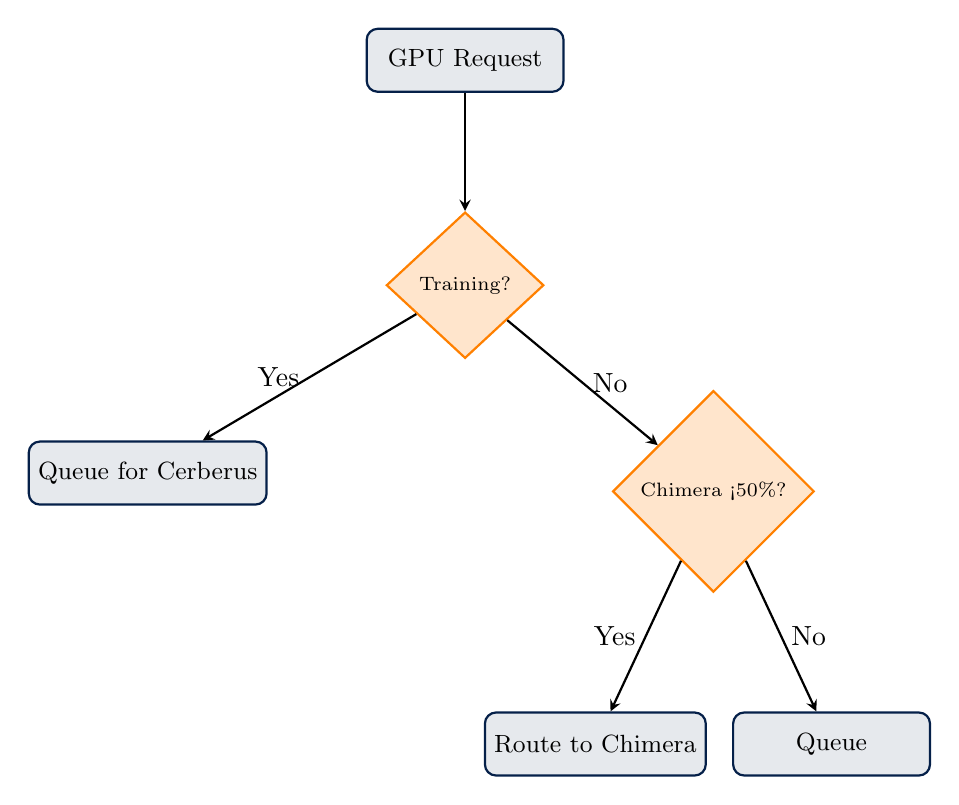
\begin{tikzpicture}[
    node distance=1.5cm,
    box/.style={rectangle, draw=hydra-blue, thick, minimum width=2.5cm, minimum height=0.8cm, fill=hydra-blue!10, rounded corners, font=\small},
    decision/.style={diamond, draw=orange, thick, minimum width=2cm, minimum height=1cm, fill=orange!20, font=\scriptsize},
    arrow/.style={->, >=stealth, thick}
]

\node[box] (request) {GPU Request};
\node[decision, below=of request] (type) {Training?};
\node[box, below left=1.5cm and 2cm of type] (cerberus) {Queue for Cerberus};
\node[decision, below right=1.5cm and 2cm of type] (util) {Chimera <50\%?};
\node[box, below=of util, xshift=-1.5cm] (chimera) {Route to Chimera};
\node[box, below=of util, xshift=1.5cm] (queue) {Queue};

\draw[arrow] (request) -- (type);
\draw[arrow] (type) -- node[left] {Yes} (cerberus);
\draw[arrow] (type) -- node[right] {No} (util);
\draw[arrow] (util) -- node[left] {Yes} (chimera);
\draw[arrow] (util) -- node[right] {No} (queue);

\end{tikzpicture}
\caption{GPU Request Routing Flow}
\end{figure}

\subsection{Migration Actions}

\begin{actionbox}
\textbf{Q.1 Container Migration Script}
\begin{itemize}[noitemsep]
    \item Export container from source node (docker export)
    \item Transfer to /tank/staging via NFS
    \item Import on target GPU node (docker import)
    \item Start with GPU runtime flags
\end{itemize}
\end{actionbox}

\begin{actionbox}
\textbf{Q.2 Simple Queue Manager}
\begin{itemize}[noitemsep]
    \item Track pending GPU requests in SQLite database
    \item Monitor GPU utilization on both nodes
    \item Process queue when capacity available
    \item Notify users via email when job starts
\end{itemize}
\end{actionbox}

\begin{actionbox}
\textbf{Q.3 Dashboard GPU Request Form}
\begin{itemize}[noitemsep]
    \item Add GPU request form to student dashboard
    \item Fields: container name, GPU type preference, duration estimate
    \item Submit to queue manager
    \item Display queue position and estimated wait time
\end{itemize}
\end{actionbox}

% =============================================================================
\section{Implementation Timeline}
% =============================================================================

\subsection{Phase 0: Pre-Migration Backup (Day 0)}
\begin{itemize}[label=$\square$]
    \item Verify Chimera /data has space (3.5TB)
    \item Create backup directories at /data/backups/
    \item Backup Hydra: /home, databases, Docker volumes
    \item Backup Chimera: /home, Ollama models, Docker volumes
    \item Backup Cerberus: /home, /etc
    \item Verify all backups completed successfully
\end{itemize}

\subsection{Phase 1: Hydra Storage (Day 1)}
\begin{itemize}[label=$\square$]
    \item Verify 6$\times$7TB drives present
    \item Install ZFS
    \item Create RAID-10 pool (3 mirror pairs)
    \item Format sdh (1.1TB) for daily OS backups
    \item Create datasets: active, inactive, staging
    \item Configure NFS exports
    \item Setup daily backup cron job
    \item Setup cluster aliases
    \item Setup centralized logging
    \item Verify Phase 1 complete
\end{itemize}

\subsection{Phase 2: GPU Node Storage (Day 2)}
\begin{itemize}[label=$\square$]
    \item Chimera: Verify drive layout
    \item Chimera: Test drive speeds
    \item Chimera: Configure Ollama on fast NVMe
    \item Chimera: Verify NVIDIA drivers
    \item Chimera: Verify Phase 2A complete
    \item Cerberus: Verify drive layout
    \item Cerberus: Format nvme1n1 for /models
    \item Cerberus: Configure Ollama
    \item Cerberus: Verify NVIDIA drivers
    \item Cerberus: Verify Phase 2B complete
\end{itemize}

\subsection{Phase 2C: Open WebUI Multi-Node (Day 2)}
\begin{itemize}[label=$\square$]
    \item Install Ollama on Chimera (models on fast NVMe)
    \item Install Ollama on Cerberus (models at /models)
    \item Pull models on both nodes
    \item Configure Open WebUI with both Ollama endpoints
    \item Verify both nodes accessible
    \item Test inference from Open WebUI
\end{itemize}

\subsection{Phase 3: RKE2 Deployment (Day 3)}
\begin{itemize}[label=$\square$]
    \item Install RKE2 server on Hydra
    \item Configure and start RKE2 server
    \item Retrieve node token
    \item Install RKE2 agent on Chimera
    \item Install RKE2 agent on Cerberus
    \item Configure kubectl access
    \item Install NVIDIA device plugin
    \item Verify all nodes Ready with GPUs
\end{itemize}

% =============================================================================
\section{Risk Assessment}
% =============================================================================

\begin{table}[H]
\centering
\caption{Risk Matrix}
\begin{tabular}{@{}p{4cm}lp{6cm}@{}}
\toprule
\textbf{Risk} & \textbf{Severity} & \textbf{Mitigation} \\
\midrule
Data loss during migration & High & Complete backups before any changes \\
Drive failure in RAID-10 & Medium & Can lose 1 drive per mirror; maintain hot spare \\
Slow /data performance & Medium & Never use for active workloads; NVMe only \\
GPU driver incompatibility & Low & Test on one node before cluster-wide deploy \\
NFS performance issues & Low & 10GbE network; async exports; local staging \\
\bottomrule
\end{tabular}
\end{table}

% =============================================================================
\section{Future Enhancements}
% =============================================================================

\begin{itemize}
    \item \textbf{Student Self-Service Portal:} Web interface for GPU access requests
    \item \textbf{Monitoring Dashboard:} Grafana dashboards for GPU/storage metrics
    \item \textbf{Automated Scaling:} Scale containers based on GPU utilization
    \item \textbf{InfiniBand Integration:} RDMA for distributed training workloads
    \item \textbf{Model Registry:} Centralized model versioning and deployment
\end{itemize}

% =============================================================================
\section{Appendix: Technology References}
% =============================================================================

\begin{table}[H]
\centering
\caption{Technology Documentation}
\begin{tabular}{@{}ll@{}}
\toprule
\textbf{Technology} & \textbf{Documentation URL} \\
\midrule
ZFS on Linux & https://openzfs.github.io/openzfs-docs/ \\
RKE2 & https://docs.rke2.io/ \\
NVIDIA Device Plugin & https://github.com/NVIDIA/k8s-device-plugin \\
Ollama & https://ollama.com/docs \\
Open WebUI & https://docs.openwebui.com/ \\
\bottomrule
\end{tabular}
\end{table}

\end{document}
